\documentclass[a4paper]{article}

%% Language and font encodings
\usepackage[english]{babel}
\usepackage[utf8x]{inputenc}
\usepackage[T1]{fontenc}

%% Sets page size and margins
\usepackage[a4paper,top=2cm,bottom=2cm,left=2cm,right=2cm,marginparwidth=2.75cm]{geometry}

%% Useful packages
\usepackage{amsmath}
\usepackage{graphicx}
\usepackage[colorinlistoftodos]{todonotes}
\usepackage[colorlinks=true, allcolors=blue]{hyperref}

%% Ammar Packages
\usepackage{float}
\usepackage{algpseudocode}
\usepackage{enumitem}

\title{ROB537: HW3}
\author{Ammar Kothari}
\date{}
\begin{document}
\maketitle


\section{Introduction}
Reinforcement learning is the ability to learn from the enviornment.  With a reward signal, an agent can figure out what actions are best to achieve the reward.  The key insight is to evaluate the value of a given conditions.  In this assignment, associating values with only an action and associating values with a state action pair are examined.  The agent trained with Q-learning which uses state action pairs achieves near optimal performance on the grid world domain.  The action value learner which only uses actions achieves good peformance on the N-armed bandit problem. 

%!TEX root = ./HW3.tex

\section{Bandit Problem}
A 10 step and 100 step version of the Bandit Problem were tested.  The same total number of steps was taken, 10,000 steps, but the episode resets occured depnding on the step length of an episode.  The solution quality for the 100 step agent is similar to the 10 step problem.

\subsection{Problem Description}
The goal for the bandit problem is to maximize the expected return given a set of slot machines that give a reward.  In this test, the rewards have a gaussian distrubution and is different for each slot machine.  The number of steps is the number of steps allowed before the situation is reset.  For the Bandit Problem, the initial state is with the accumulated reward as zero.

\subsection{Results}
An action value learning agent is used in both cases.  Figure \ref{fig:Bandit20} and Figure {\ref{fig:Bandit0} shows the expected values as estimated by the learning for both episode lenghts with two different exploration amounts along with the actual distribution of the learners.  Table \ref{tab:Bandit} shows statistics of the reward obtained by the agents.

\begin{table}[]
\centering
\begin{tabular}{|c|c|c|c|}
\hline
Steps & Exploration & Reward & StDev \\ \hline
10    & 0.2         & 0.914  & 1.24  \\ \hline
100   & 0.2         & 1.49   & 0.58  \\ \hline
10    & 0.0         & 1.14   & 0.94  \\ \hline
100   & 0.0         & 0.93   & 1.87  \\ \hline
\end{tabular}
\caption{Results for different tests for Bandit Problem with an Action Value learner}
\label{tab:Bandit}
\end{table}

\subsection{Analysis}
All version struggle to approximate the true distribution.  This can be caused by an insufficient number of samples.  With increased exploration, the true values are generally approximated better.  For action 2 and no exploration, appears to be close to the true value while the many of the other estimates are not close to approximating the true distribution.  

% image of bandit comparison for 20% exploration
\begin{figure}[h]
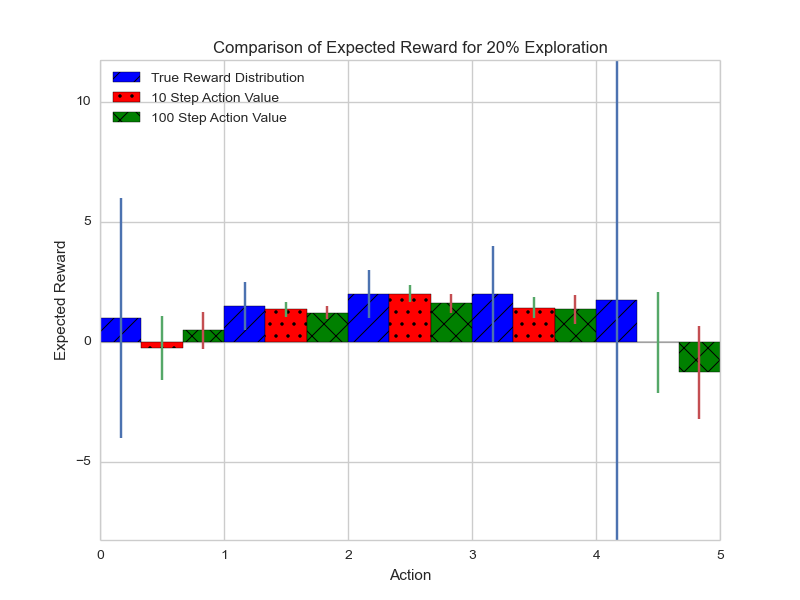
\includegraphics[width=\linewidth]{Bandit20.png}
\caption{Comparison of Action Value tables between selection for 10 steps and 100 steps for an action-value learner with 20\% epsilon greedy exploration  on a multiarmed bandit problem.}
\label{fig:Bandit20}
\end{figure}

% image of bandit comparison for 0% exploration
\begin{figure}[h]
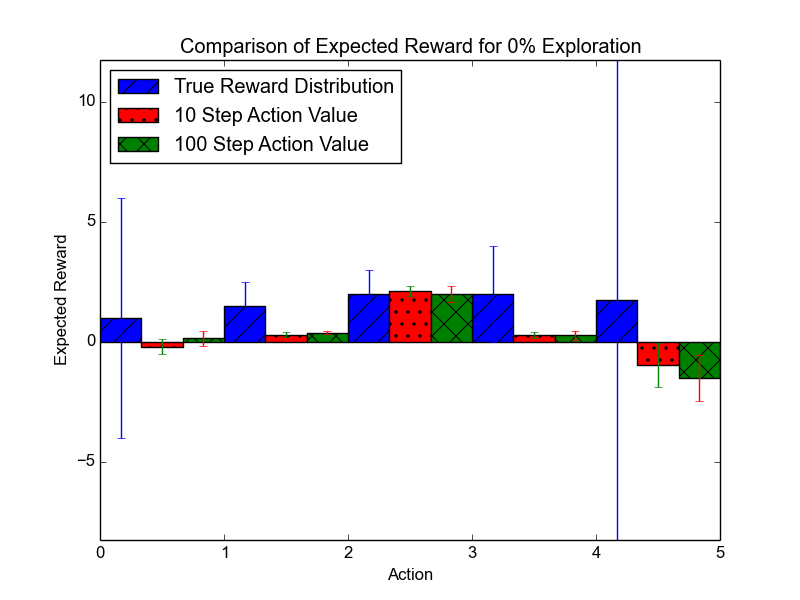
\includegraphics[width=\linewidth]{Bandit0.png}
\caption{Comparison of Action Value tables between selection for 10 steps and 100 steps for an action-value learner with 0\% epsilon greedy exploration  on a multiarmed bandit problem.}
\label{fig:Bandit0}
\end{figure}

%!TEX root = ./HW3.tex

\section{Grid World}
For grid world, two different types of learners are tested.  The first only estimates the expected reward of actions.  The second estimates the rewards based on state action pairs.  The performance of the state action pair is better.

\subsection{Problem Description}
In Grid World, the agent is spawned at a random location in the world.  The goal is a location on the map.  Every location that is not the goal gives a reward of -1 and the goal gives a reward of 100.  The length of an episode is 100 steps.  At the end of an episode, the location of the agent is randomly placed on the map.

\subsection{Results}
The learning progression is shown in Figure \ref{fig:GridLearn}.  The Q-Learning agent performs better than the Action Value agent.  An example trajector after training is completed is shown in \ref{}.

\subsection{Analysis}
Action Value learning basically learns how to stay in the middle of the map and rarely moves left.  This is because at every spot, moving left is not the optimal action.  The action value learner does not associate rewards with state and as a result, moves around the center of the map without moving towards the goal.  This is shown by the example trajectories in Figure \ref{}.

Q learning performs much better.  The trade off is that significantly more information must be stored compared to the Action Value learner.


\begin{figure}[h]
\includegraphics{AVGrid.png}
\caption{Learning progress of both agents on grid world.  Q learning agent is able to improve over the course of training, where as the Action Value agent never improves significantly.}
\label{fig:GriudLearn}
\end{figure}

\begin{figure}[h]
\includegraphics{AVGridSolution.png}
\caption{Action value table quiver plot for epsilon greedy agent for 20 steps.  Arrows are weighted average of the best action at that state.}
\label{fig:AVGridSolution}
\end{figure}

%!TEX root = ./HW3.tex



\begin{figure}[h]
\includegraphics{QLearnerProgress.png}
\caption{Q learner learning progression.}
\label{fig:QLearnerProgress}
\end{figure}


\begin{figure}[h]
\includegraphics{QGridSolution.png}
\caption{Q table quiver plot for epsilon greedy agent for 20 steps.  Arrows are weighted average of the best action at that state.}
\label{fig:QGridSolution}
\end{figure}

\section{Conclusion}
In general, Q learning is the more effective agent.  If the problem has only one state, an Action Value learning, which is a single state case of Q learning, will be able to solve the problem.  For simple grid world problems, Q-learning is able to find the optimal path from any location on the map to the reward.

\end{document}	